  \chapter{Planificacion}
  \label{chap:planificacion}


    \section{Analisis}
    \label{sec:Analisis}

      % La programacion extrema no contempla especificamente el diseno de casos de uso
      Dentro del analisis se realizo el diseno de Casos de Uso como parte del proceso para entender el comportamiento del sistema. \cite{casos_uso}
  %

  \begin{figure}[H]
    \begin{center}
      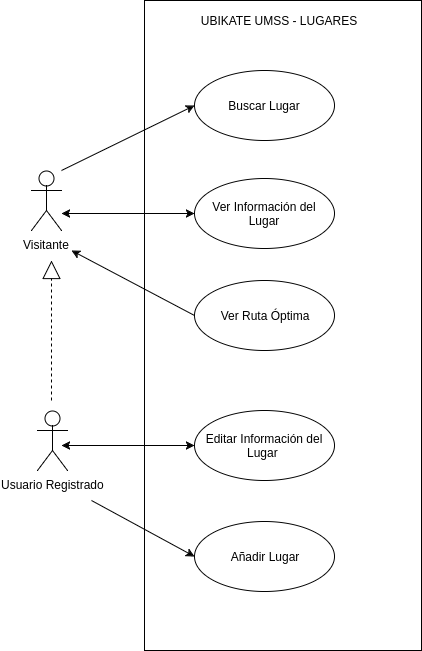
\includegraphics[width=0.45\textwidth]{casos_uso/cu_lugares}
    \end{center}
    \caption{Diagrama Casos de Uso - Gestion de Lugares }
    \label{fig:cu_lugares}
    \caption*{Fuente: Elaboración propia}
  \end{figure}

  \begin{table}[H]
  \begin{center}
    \begin{tabularx}{0.75\textwidth}{ X X  }
      \toprule
      \multicolumn{2}{l}{\textbf{Caso de Uso:} Buscar Lugar} \\
      \multicolumn{2}{l}{\textbf{Actor:} Visitante} \\
      \multicolumn{2}{l}{\textbf{Precondición:} El Visitante accede al sistema.} \\
      \addlinespace
      \textbf{Secuencia Principal} & \textbf{Alternativas} \\
      \midrule
      1. El Visitante accede a la sección de ``Lugares''. \\
      \addlinespace
      2. El visitante ingresa el nombre del lugar en un \emph{search box}.  \\
      \addlinespace
      3. El Visitante ve la lista de Lugares registrados que coinciden con la búsqueda. &
      3.1 El lugar no existe en la base de datos, retorna una lista vacía. \\

      \midrule
      \multicolumn{2}{l}{\textbf{Postcondición:} El Visitante encuentra un lugar} \\

      \bottomrule
    \end{tabularx}
    \caption{Caso de Uso - Buscar Lugar}
    \label{tab:cu_buscar_lugar}
  \end{center}
\end{table}


% \begin{table}[H]
%   \begin{center}
%     \begin{tabularx}{0.75\textwidth}{  L{3cm} X  }
%       \toprule
%       \textbf{Caso de Uso:} & Buscar Lugar \\
%       \textbf{Actor:} & Visitante \\
%       \textbf{Precondición:} & El Visitante accede al sistema. \\
%       \textbf{Secuencia Principal:} & 1. El Visitante accede a la sección de ``Lugares''. \\
%       \addlinespace
%       & 2. El visitante ingresa el nombre del lugar en un \emph{search box}.  \\
%       \addlinespace
%       & 3. El Visitante ve la lista de Lugares registrados que coinciden con la búsqueda. \\
%
%       \addlinespace
%       \textbf{Postcondición:} & El Visitante encuentra un lugar. \\
%       \bottomrule
%     \end{tabularx}
%     \caption{Caso de Uso - Buscar Lugar}
%     \label{tab:cu_buscar_lugar}
%   \end{center}
% \end{table}




\begin{table}[H]
  \begin{center}
    \begin{tabularx}{0.75\textwidth}{ X X  }
      \toprule
      \multicolumn{2}{l}{\textbf{Caso de Uso:} Ver Información del Lugar} \\
      \multicolumn{2}{l}{\textbf{Actor:} Visitante} \\
      \multicolumn{2}{l}{\textbf{Precondición:} El Visitante ha buscado un lugar} \\
      \addlinespace
      \textbf{Secuencia Principal} & \textbf{Alternativas} \\
      \midrule
      1. El Visitante hace un tap sobre el nombre del lugar en la lista de búsqueda. \\
      \addlinespace
      2. El visitante puede ver una imagen del lugar. &
      2.1. Si el lugar no tiene una imagen asociada, se desplegará una imagen genérica de la UMSS.\\
      \addlinespace
      3. El Visitante ve la descripción del lugar. & \\

      \midrule
      \multicolumn{2}{l}{\textbf{Postcondición:} El Visitante puede ver la información del lugar.} \\
      \bottomrule
    \end{tabularx}
    \caption{Caso de Uso - Ver Información del lugar}
    \label{tab:cu_info_lugar}
  \end{center}
\end{table}


\begin{table}[H]
  \begin{center}
    \begin{tabularx}{0.75\textwidth}{ X X  }
      \toprule
      \multicolumn{2}{l}{\textbf{Caso de Uso:} Ver Ruta Óptima} \\
      \multicolumn{2}{l}{\textbf{Actor:} Visitante} \\
      \multicolumn{2}{l}{\textbf{Precondición:} El Visitante observa la información del lugar.} \\
      \addlinespace
      \textbf{Secuencia Principal} & \textbf{Alternativas} \\
      \midrule
      1. El Visitante selecciona el botón que muestra la ruta más corta al lugar. & \\
      \addlinespace
      2. El sistema pregunta si el usuario quiere compartir su ubicación geográfica. & \\
      \addlinespace
      3. El Visitante acepta la pregunta. &
      3.1. Si el usuario niega la pregunta, el sistema no puede mostrar la ruta óptima. \\

      \midrule
      \multicolumn{2}{L{11cm}}{\textbf{Postcondición:} El Visitante ve un mapa con un marcador y una línea mostrando la ruta óptima. } \\

      \bottomrule
    \end{tabularx}
    \caption{Caso de Uso - Ver Ruta Óptima}
    \label{tab:cu_ruta_optima}
  \end{center}
\end{table}




% \begin{table}[H]
%   \begin{center}
%     \begin{tabularx}{0.75\textwidth}{ X X  }
%       \toprule
%       \multicolumn{2}{l}{\textbf{Caso de Uso:} Ver Ruta Óptima} \\
%       \multicolumn{2}{l}{\textbf{Actor:} Visitante} \\
%       \multicolumn{2}{l}{\textbf{Precondición:} El Visitante está viendo la información del lugar.} \\
%       \addlinespace
%       \textbf{Secuencia Principal} & \textbf{Alternativas} \\
%       \midrule
%       1. El Visitante selecciona el botón que muestra la ruta más corta al lugar. & \\
%       \addlinespace
%       2. El sistema pregunta si el usuario quiere compartir su ubicación geográfica. & \\
%       \addlinespace
%       3. El Visitante acepta la pregunta. &
%       3.1. Si el usuario niega la pregunta, el sistema no puede mostrar la ruta óptima.\\
%
%       \midrule
%       \multicolumn{2}{l}{\textbf{Postcondición:} El Visitante ve un mapa con el lugar marcado y una línea que conecta la posición actual del usuario con el lugar.} \\
%
%       \bottomrule
%     \end{tabularx}
%     \caption{Caso de Uso - Ver Ruta Óptima}
%     \label{tab:cu_ruta_optima}
%   \end{center}
% \end{table}
%
%



\begin{table}[H]
  \begin{center}
    \begin{tabularx}{0.75\textwidth}{ X X  }
      \toprule
      \multicolumn{2}{l}{\textbf{Caso de Uso:} Editar Información del Lugar} \\
      \multicolumn{2}{l}{\textbf{Actor:} Visitante Registrado} \\
      \multicolumn{2}{L{12cm}}{\textbf{Precondición:} El Visitante Registrado esta viendo la información del lugar.} \\
      \addlinespace
      \textbf{Secuencia Principal} & \textbf{Alternativas} \\
      \midrule
      1. El Visitante Registrado selecciona el boton de Edicion. \\
      \addlinespace
      2. El sistema muestra un formulario con la información actual del Lugar.& \\
      \addlinespace
      3. El Visitante Registrado selecciona el botón ``Aceptar''. & \\


      \midrule
      \multicolumn{2}{L{11cm}}{\textbf{Postcondición:} El sistema muestra la información del Lugar actualizada.} \\

      \bottomrule
    \end{tabularx}
    \caption{Caso de Uso - Editar Información del Lugar}
    \label{tab:cu_edit_place}
  \end{center}
\end{table}


\begin{table}[H]
  \begin{center}
    \begin{tabularx}{0.75\textwidth}{ X X }
      \toprule
      \multicolumn{2}{l}{\textbf{Caso de Uso:} Añadir Lugar} \\
      \multicolumn{2}{l}{\textbf{Actor:} Visitante Registrado} \\
      \multicolumn{2}{L{12cm}}{\textbf{Precondición:} El Visitante Registrado necesita desplazarse hasta el lugar para añadirlo.} \\
      \addlinespace
      \textbf{Secuencia Principal} & \textbf{Alternativas} \\
      \midrule
      1. El Visitante Registrado ha accedido a la sección de ``Lugares''. & \\
      \addlinespace
      2. El Visitante Registrado puede ver un botón de adición al final de la lista de lugares. &\\
      \addlinespace
      3. El sistema pregunta si se desea compartir la ubicación geográfica.
      \addlinespace
      3. El Visitante Registrado acepta la pregunta. &
      3.1. El visitante niega la pregunta.\\
      \addlinespace
      4. El Visitante Registrado ve un formulario para ingresar la información del lugar. &
      4.1. El Visitante Registrado no puede anadir un nuevo lugar. \\
      \addlinespace
      5. El Visitante Registrado acepta el formulario. & \\

      \midrule
      \multicolumn{2}{l}{\textbf{Postcondición:} El sistema muestra el lugar en la lista de lugares.} \\

      \bottomrule
    \end{tabularx}
    \caption{Caso de Uso - Añadir Lugar}
    \label{tab:cu_add_place}
  \end{center}
\end{table}


  \begin{figure}[H]
    \begin{center}
      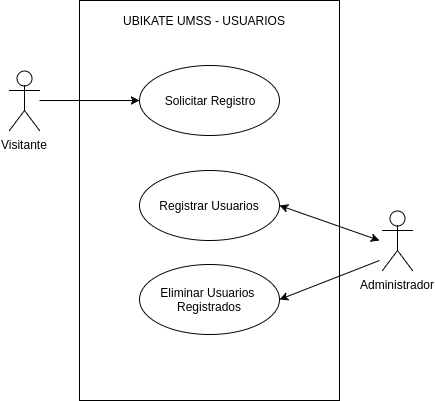
\includegraphics[width=0.45\textwidth]{casos_uso/cu_usuarios}
    \end{center}
    \caption{Diagrama Casos de Uso - Gestion de Usuarios }
    \label{fig:cu_usuarios}
    \caption*{Fuente: Elaboración propia}
  \end{figure}

  \begin{table}[H]
  \begin{center}
    \begin{tabularx}{0.75\textwidth}{ X X  }
      \toprule
      \multicolumn{2}{l}{\textbf{Caso de Uso:} Solicitar Registro} \\
      \multicolumn{2}{l}{\textbf{Actor:} Visitante} \\
      \multicolumn{2}{l}{\textbf{Precondición:} El Visitante accede al sistema.} \\
      \addlinespace
      \textbf{Secuencia Principal} & \textbf{Alternativas} \\
      \midrule
      1. El Visitante accede a la sección de ``Registro''. \\
      \addlinespace
      2. El visitante ingresa su nombre y una direccion email.  \\

      \midrule
      \multicolumn{2}{l}{\textbf{Postcondición:} El Visitante ve un mensaje de confirmacion} \\

      \bottomrule
    \end{tabularx}
    \caption{Caso de Uso - Solicitar Registro}
    \label{tab:cu_solicitar_registro}
  \end{center}
\end{table}


\begin{table}[H]
  \begin{center}
    \begin{tabularx}{0.75\textwidth}{ X X  }
      \toprule
      \multicolumn{2}{l}{\textbf{Caso de Uso:} Registrar Usuario} \\
      \multicolumn{2}{l}{\textbf{Actor:} Administrador} \\
      \multicolumn{2}{l}{\textbf{Precondición:} El Administrador accede al sistema.} \\
      \addlinespace
      \textbf{Secuencia Principal} & \textbf{Alternativas} \\
      \midrule
      1. El Administrador accede a la sección de ``Registro de Usuarios''. \\
      \addlinespace
      2. El Administrador ve una lista con de usuarios a registrar.  \\
      \addlinespace
      3. El Administrador acepta el registro del usuario.  \\
      \addlinespace
      3. El sistema manda un email con instrucciones al usuario.  \\
      \addlinespace
      4. Un mensaje confirmando el envio del email es mostrado. & 4.1. Si el email no existe, un mensaje es mostrado y el registro del usuario es cancelado.  \\

      \midrule
      \multicolumn{2}{L{12cm}}{\textbf{Postcondición:} El Visitante deberia recibir un email con instrucciones de registro.} \\

      \bottomrule
    \end{tabularx}
    \caption{Caso de Uso - Registrar Usuario}
    \label{tab:cu_solicitar_registro}
  \end{center}
\end{table}



\begin{table}[H]
  \begin{center}
    \begin{tabularx}{0.75\textwidth}{ X X  }
      \toprule
      \multicolumn{2}{l}{\textbf{Caso de Uso:} Eliminar Usuarios Registrados} \\
      \multicolumn{2}{l}{\textbf{Actor:} Administrador} \\
      \multicolumn{2}{l}{\textbf{Precondición:} El Administrador accede al sistema.} \\
      \addlinespace
      \textbf{Secuencia Principal} & \textbf{Alternativas} \\
      \midrule
      1. El Administrador accede a la sección de ``Usuarios Registrados''. \\
      \addlinespace
      2. El Administrador elimina un usuario registrado.  \\
      \addlinespace
      3. Un mensaje confirmando la eliminacion del usuario es mostrado.\\

      \midrule
      \multicolumn{2}{L{11.5cm}}{\textbf{Postcondición:} El Usuario eliminado ya no deberia ser visible en la lista de Usuarios registrados.} \\

      \bottomrule
    \end{tabularx}
    \caption{Caso de Uso - Eliminar Usuarios Registrados}
    \label{tab:cu_solicitar_registro}
  \end{center}
\end{table}



  \begin{figure}[H]
    \begin{center}
      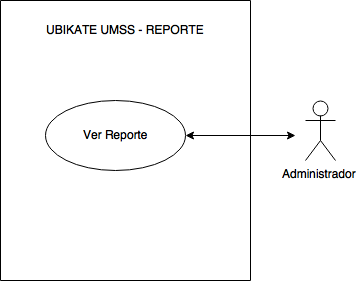
\includegraphics[width=0.45\textwidth]{casos_uso/cu_reporte}
    \end{center}
    \caption{Diagrama Casos de Uso - Reporte }
    \label{fig:cu_reporte}
    \caption*{Fuente: Elaboración propia}
  \end{figure}

  \begin{table}[H]
  \begin{center}
    \begin{tabularx}{0.75\textwidth}{ X X  }
      \toprule
      \multicolumn{2}{l}{\textbf{Caso de Uso:} Ver Reporte} \\
      \multicolumn{2}{l}{\textbf{Actor:} Administrador} \\
      \multicolumn{2}{l}{\textbf{Precondición:} El Administrador accede al sistema.} \\
      \addlinespace
      \textbf{Secuencia Principal} & \textbf{Alternativas} \\
      \midrule
      1. El Administrador accede a la sección de ``Reporte''. \\
      \addlinespace
      2. El Sistema genera una grafica en relacion a los lugares mas visitados.  \\

      % \midrule
      % \multicolumn{2}{l}{\textbf{Postcondición:} El Visitante encuentra un lugar} \\

      \bottomrule
    \end{tabularx}
    \caption{Caso de Uso - Ver Reporte}
    \label{tab:cu_ver_reporte}
  \end{center}
\end{table}



  % Siguiendo la metodología XP, el presente proyecto de grado debe empezar por la primera etapa del Planning Game.\\


  % Exploración - Entrega y estimación de las historias de usuario

    \section{Historias de Usuario}
    \label{sec:historias_de_usuario}

      Una vez realizado los casos de uso se procede con las Historias de Usario

      % % user_story_01
% % \begin{table}[!ht]
% \begin{table}[H]
%   \begin{center}
%     \begin{tabular}{ L{3cm}  L{8cm} }
%       \toprule
%         \textbf{Historia} US01 &
%         % \textbf{Esfuerzo} 5 puntos \\
%         \makebox[6cm][r]{\textbf{Esfuerzo} 8 puntos} \\
%         % \makebox[4cm][r]{\textbf{Estimación} 3 días} \\
%
%       \midrule
%       \multirow{3}{*}{\textbf{Descripción}}
%         & Yo como visitante\\
%         & Deseo registrarme en el sistema\\
%         & Para poder acceder al sistema\\
%       \midrule
%         \multirow{3}{3cm}{\textbf{Criterios de Aceptación}}
%         & Quiero ver fácilmente que no estoy registrado\\
%         & Quiero que el registro solamente me pida un nombre de usuario y un password\\
%         & Quiero ver que al estar registrado pueda acceder a los lugares\\
%       \bottomrule
%     \end{tabular}
%     \caption{Historia de Usuario - US01}
%     \label{tab:user_story_01}
%   \end{center}
% \end{table}

% user_story_02

% user_story_03

\begin{table}[H]
  \begin{center}
    \begin{tabular}{ L{3cm}  L{8cm} }
      \toprule
        \textbf{Código:} & US01 \\
        \textbf{Prioridad:} & Alta \\
        \textbf{Riesgo:} & Alta \\

        % \addlinespace
      \midrule
        \multirow{3}{*}{\textbf{Descripción:}}
        & Yo como visitante\\
        & Deseo ver una lista de lugares \\
        % & Deseo ingresar el nombre de un lugar\\
        & Para encontrar el lugar al que deseo ir\\
        \addlinespace
      % \midrule
        \multirow{3}{3cm}{\textbf{Criterios de Aceptación:}}
        & Quiero tener los lugares en una base de datos \\
        & Quiero ver una lista de lugares\\
        & Quiero filtrar la lista de lugares por el nombre o parte de este\\
        % & Quiero encontrar un lugar
        % & Quiero encontrar un lugar y poder ver su información\\
      \bottomrule
    \end{tabular}
    \caption{Historia de Usuario - US01}
    \label{tab:user_story_01}
  \end{center}
\end{table}

\begin{table}[H]
  \begin{center}
    \begin{tabular}{ L{3cm}  L{8cm} }
      \toprule
        \textbf{Historia} US02 &
        % \textbf{Esfuerzo} 5 puntos \\
        \makebox[6cm][r]{\textbf{Esfuerzo} 8 puntos} \\
        % \makebox[4cm][r]{\textbf{Estimación} 3 días} \\

      \midrule
        \multirow{3}{*}{\textbf{Descripción}}
        & Yo como visitante\\
        & Deseo ver la información de un lugar\\
        & Para decidir si es el lugar que estoy buscando\\
      \midrule
        \multirow{3}{3cm}{\textbf{Criterios de Aceptación}}
        & Quiero leer una descripción del lugar\\
        & Quiero ver un teléfono asociado al lugar\\
        & Quiero ver en qué piso se encuentra el lugar\\
      \bottomrule
    \end{tabular}
    \caption{Historia de Usuario - US02}
    \label{tab:user_story_02}
  \end{center}
\end{table}



% user_story_03

\begin{table}[H]
  \begin{center}
    \begin{tabular}{ L{3cm}  L{8cm} }
      \toprule
        \textbf{Historia} US03 &
        % \textbf{Esfuerzo} 5 puntos \\
        \makebox[6cm][r]{\textbf{Esfuerzo} 8 puntos} \\
        % \makebox[4cm][r]{\textbf{Estimación} 3 días} \\

      \midrule
        \multirow{3}{*}{\textbf{Descripción}}
        & Yo como visitante\\
        & Deseo ver el lugar en un mapa\\
        & Para saber en que parte del campus se encuentra el lugar\\
      \midrule
        \multirow{3}{3cm}{\textbf{Criterios de Aceptación}}
        & Deseo ver sobre un mapa un punto del lugar buscado a donde quiero ir\\
        & Quiero ver un marcador sobre el lugar que estoy buscando con alguna información para asegurarme que es a donde quiero ir\\

      \bottomrule
    \end{tabular}
    \caption{Historia de Usuario - US03}
    \label{tab:user_story_03}
  \end{center}
\end{table}


% user_story_04

\begin{table}[H]
  \begin{center}
    \begin{tabular}{ L{3cm}  L{8cm} }
      \toprule
        \textbf{Historia} US04 &
        % \textbf{Esfuerzo} 5 puntos \\
        \makebox[6cm][r]{\textbf{Esfuerzo} 8 puntos} \\
        % \makebox[4cm][r]{\textbf{Estimación} 3 días} \\

      \midrule
        \multirow{3}{*}{\textbf{Descripción}}
        & Yo como visitante\\
        & Deseo ver una ruta sobre el mapa\\
        & Para encontrar el lugar de forma rapida\\
      \midrule
        \multirow{1}{3cm}{\textbf{Criterios de Aceptación}}
        & Deseo ver sobre un mapa un punto del lugar actual donde me encuentro\\

        & Deseo ver una línea roja que muestre la ruta más corta para llegar de mi ubicación al lugar donde quiero ir\\

      \bottomrule
    \end{tabular}
    \caption{Historia de Usuario - US04}
    \label{tab:user_story_04}
  \end{center}
\end{table}


% user_story_04

\begin{table}[H]
  \begin{center}
    \begin{tabular}{ L{3cm}  L{8cm} }
      \toprule
        \textbf{Historia} US05 &
        % \textbf{Esfuerzo} 5 puntos \\
        \makebox[6cm][r]{\textbf{Esfuerzo} 8 puntos} \\
        % \makebox[4cm][r]{\textbf{Estimación} 3 días} \\

      \midrule
        \multirow{3}{*}{\textbf{Descripción}}
        & Yo como visitante\\
        & Deseo registrarme\\
        & Para tener mas opciones dentro el sistema\\
      \midrule
        \multirow{3}{3cm}{\textbf{Criterios de Aceptación}}
        & Quiero ver un formulario donde me pueda registrar.\\
        & Una vez registrado quiero poder ingresar al sistema con mis credenciales.\\
        & Quiero ver tener la posibilidad de editar mis datos.\\
      \bottomrule
    \end{tabular}
    \caption{Historia de Usuario - US05}
    \label{tab:user_story_05}
  \end{center}
\end{table}



% user_story_05

\begin{table}[H]
  \begin{center}
    \begin{tabular}{ L{3cm}  L{8cm} }
      \toprule
        \textbf{Historia} US06 &
        % \textbf{Esfuerzo} 5 puntos \\
        \makebox[6cm][r]{\textbf{Esfuerzo} 8 puntos} \\
        % \makebox[4cm][r]{\textbf{Estimación} 3 días} \\

      \midrule
        \multirow{3}{*}{\textbf{Descripción}}
        & Yo como usuario registrado\\
        & Deseo añadir más lugares al sistema\\
        & Para mejorar los criterios de busqueda\\
      \midrule
        \multirow{3}{3cm}{\textbf{Criterios de Aceptación}}
        & Quiero que sea posible anadir un lugar si no lo encuentro en la lista de lugares\\
        & Quiero ver un formulario para poder ingresar los datos de un nuevo lugar.\\
        & Quiero pararme cerca o en el lugar que necesito añadir para geo-referenciarlo\\
        % & Al añadir un lugar necesito ingresar alguna descripción y/o teléfono si fuera necesario\\
      \bottomrule
    \end{tabular}
    \caption{Historia de Usuario - US06}
    \label{tab:user_story_06}
  \end{center}
\end{table}



% user_story_06

\begin{table}[H]
  \begin{center}
    \begin{tabular}{ L{3cm}  L{8cm} }
      \toprule
        \textbf{Historia} US07 &
        % \textbf{Esfuerzo} 5 puntos \\
        \makebox[6cm][r]{\textbf{Esfuerzo} 8 puntos} \\
        % \makebox[4cm][r]{\textbf{Estimación} 3 días} \\

      \midrule
        \multirow{3}{*}{\textbf{Descripción}}
        & Yo como usuario registrado\\
        & Deseo editar la información de un lugar\\
        & Para mejorar o corregir la información de ese lugar\\
      \midrule
        \multirow{3}{3cm}{\textbf{Criterios de Aceptación}}
        & Al entrar a la información de un lugar quiero ser el único que vea un icono para poder entrar a la edición de los datos\\
        & Quiero acceder a un formulario que muestre la información actual del lugar y poder editar la información mostrada\\

      \bottomrule
    \end{tabular}
    \caption{Historia de Usuario - US07}
    \label{tab:user_story_07}
  \end{center}
\end{table}

% user_story_07

\begin{table}[H]
  \begin{center}
    \begin{tabular}{ L{3cm}  L{8cm} }
      \toprule
        \textbf{Historia} US08 &
        % \textbf{Esfuerzo} 5 puntos \\
        \makebox[6cm][r]{\textbf{Esfuerzo} 8 puntos} \\
        % \makebox[4cm][r]{\textbf{Estimación} 3 días} \\

      \midrule
        \multirow{3}{*}{\textbf{Descripción}}
        & Yo como usuario administrador\\
        & Deseo administrar usuarios\\
        & Para anadir o remover usuarios del sistema\\
      \midrule
        \multirow{3}{3cm}{\textbf{Criterios de Aceptación}}
        & Quiero ver los usuarios que desean registrarse en el sistema\\
        & Quiero aceptar o rechazar solicitudes de registro\\
        & Quiero eliminar usuarios que no usen el sistema de forma adecuada.\\

      \bottomrule
    \end{tabular}
    \caption{Historia de Usuario - US08}
    \label{tab:user_story_08}
  \end{center}
\end{table}


% user_story_08

\begin{table}[H]
  \begin{center}
    \begin{tabular}{ L{3cm}  L{8cm} }
      \toprule
        \textbf{Historia} US09 &
        % \textbf{Esfuerzo} 5 puntos \\
        \makebox[6cm][r]{\textbf{Esfuerzo} 13 puntos} \\
        % \makebox[4cm][r]{\textbf{Estimación} 3 días} \\

      \midrule
        \multirow{3}{*}{\textbf{Descripción}}
        & Yo como usuario administrador\\
        & Deseo ver los lugares más visitados\\
        & Para obtener información y estadísticas de los lugares dentro del campus Universitario\\
      \midrule
        \multirow{3}{3cm}{\textbf{Criterios de Aceptación}}
        & Quiero apreciar de forma sencilla la cantidad de veces que los usuarios buscan un lugar\\
        & Quiero poder guardarla el reporte\\

      \bottomrule
    \end{tabular}
    \caption{Historia de Usuario - US09}
    \label{tab:user_story_09}
  \end{center}
\end{table}


    % end historias_de_usuario

    \section{Planeacion de Entregas}
    \label{sub:Planeacion de Entregas}

        A continuación el calendario de entregas del proyecto, el cual de acuerdo de las historias de usuario recogidas se estimó para unas 4 Iteraciones, y cada Iteración de 2 semanas.\\

        % \begin{table}[!ht]
%
% \end{table}
\begin{table}[H]
  \label{tab:calendario_entregas}
  \begin{center}

\begin{ganttchart}[
  canvas/.append style={fill=none, draw=black!5, line width=.75pt},
  hgrid style/.style={draw=black!5, line width=.75pt},
  vgrid={*1{draw=black!5, line width=.75pt}},
  %today=0,
  % today label=Semana 3,
  today rule/.style={
    draw=black!64,
    dash pattern=on 3.5pt off 4.5pt,
    line width=1.5pt
  },
  today label font=\small\bfseries,
  title/.style={draw=none, fill=none},
  title label font=\bfseries\footnotesize,
  title label node/.append style={below=7pt},
  include title in canvas=false,
  bar label font=\mdseries\small\color{black!70},
  bar label node/.append style={left=2cm},
  bar/.append style={draw=none, fill=black!63},
  bar incomplete/.append style={fill=barblue},
  bar progress label font=\mdseries\footnotesize\color{black!70},
  group incomplete/.append style={fill=groupblue},
    group left shift=0,
    group right shift=0,
    group height=.5,
    group peaks tip position=0,
    group label node/.append style={left=.6cm},
    group progress label font=\bfseries\small,
    link/.style={-latex, line width=1.5pt, linkred},
    link label font=\scriptsize\bfseries,
    link label node/.append style={below left=-2pt and 0pt},
  ]{1}{12}
  \gantttitle{Calendario de Entregas}{12} \\[grid]
  \gantttitle{Septiembre}{4}
  \gantttitle{Octubre}{4}
  \gantttitle{Noviembre}{4} \\
  \gantttitle[title label node/.append style={below left=7pt and -3pt}]{Semana:\quad1}{1}
  \gantttitlelist{2,...,12}{1} \\
  \ganttgroup[progress=0]{Historias de Usuario}{1}{8} \\
  \ganttbar[
    progress=0,
    name=bar1
  ]{\textbf{Iteración 1}}{1}{2} \\
  \ganttbar[
    progress=0,
    name=bar2
  ]{\textbf{Iteración 2}}{3}{4} \\
  \ganttbar[
    progress=0,
    name=bar3
  ]{\textbf{Iteración 3}}{5}{6} \\
  \ganttbar[
    progress=0,
    name=bar4
  ]{\textbf{Iteración 4}}{7}{8} \\
  % \ganttbar[
  %   progress=100,
  %   name=bar5
  % ]{\textbf{Actividad 5}}{5}{7} \\
  % \ganttbar[
  %   progress=80,
  % ]{\textbf{Actividad 6}}{8}{8} \\
  % \ganttbar[
  %   progress=49,
  % ]{\textbf{Actividad 7}}{9}{11} \\
  % \ganttmilestone{Hito 1}{11}{11}  \\
  % \ganttmilestone{Hito 2}{12}{12} \\
  %

  % \ganttmilestone{Q6 report}{24}{24} \\
  \ganttmilestone{M1: Project finished}{8}{8}

  \ganttlink[link type=f-s]{bar1}{bar2}
  \ganttlink[link type=f-s]{bar2}{bar3}
  \ganttlink[link type=f-s]{bar3}{bar4}

\end{ganttchart}

\caption{Calendario de Entregas}
\end{center}
\end{table}


        El orden de implementación y la estimación del equipo de desarrollo para completar las Historias de Usuario se pueden apreciar en la tabla \ref{tab:user_stories_order}.

        \begin{table}[H]

          \begin{center}
            \begin{tabular}{ c  c  c }
              \toprule
                \textbf{Iteración} &
                \textbf{Historia de Usuario} &
                \textbf{Estimación [dias]}\\

              \midrule
                \multirow{2}{*}{Iteración 1}
                & US02 & 6\\
                & US03 & 4\\

              \addlinespace
                Iteración 2 & US04 & 10\\

              % \midrule
              \addlinespace
                \multirow{2}{*}{Iteración 3}
                & US05 & 5\\
                & US06 & 5\\
              %
              % \midrule
              \addlinespace
                \multirow{2}{*}{Iteración 4}
                & US01 & 4\\
                & US07 & 6\\

              \bottomrule
            \end{tabular}
            \caption{Estimación de la implementación de las Historias de Usuario.}
            \label{tab:user_stories_order}
          \end{center}
        \end{table}

  % end implementacion


% end desarrollo
